\documentclass[../norme-di-progetto.tex]{subfiles}

\begin{document}

\subsection{Descrizione}%
\label{sub:processi_primari/descrizione}
Sono i processi essenziali durante il ciclo di vita del software. ISO 12207:1995 ne definisce cinque:

\begin{itemize}
  \item Acquisizione
  \item Fornitura
  \item Sviluppo
  \item Gestione operativa
  \item Manutenzione.
\end{itemize}

Di questi, noi istanziamo in maniera significativa solo i processi di fornitura e sviluppo.

\subsection{Fornitura}%
\label{sub:fornitura}

\subsubsection{Finalità}%
\label{subs:fornitura/finalita}

GruppOne istanzia il processo di fornitura per potersi aggiudicare il capitolato attraverso un accordo con il committente che ha valore contrattuale.

\subsubsection{Descrizione}%
\label{subs:fornitura/descrizione}

Il processo di fornitura concerne il rapporto tra il fornitore e il cliente, e l'amministrazione delle procedure e risorse necessarie per lo sviluppo del \textit{Piano di progetto}.

È composto da diverse attività:

\begin{itemize}
  \item Inizializzazione
  \item Preparazione della risposta
  \item Contratto
  \item Pianificazione
  \item Esecuzione e controllo
  \item Revisione e valutazione
  \item Consegna e completamento.
\end{itemize}

\subsubsection{Studio di Fattibilità}%
\label{subs:studio_di_fattibilita}

GruppOne si impegna a consegnare un documento sintetico contenente una descrizione, i pregi e le criticità riscontrati in ciascuno dei capitolati.

Lo \textit{Studio di fattibilità} è redatto dall'\glossario{amministratore} con l'aiuto degli \glossario{analisti} e ha l'obiettivo di esporre quali capitolati sono presi in considerazione e le relative motivazioni.

Il documento è così articolato:
\begin{description}
  \item [Descrizione] una breve descrizione del problema esposto dal proponente
  \item [Finalità del progetto] che cosa bisogna realizzare
  \item [Tecnologie interessate] le tecnologie da considerare in fase di sviluppo
  \item [Aspetti positivi] i pregi del capitolato
  \item [Criticità e fattori di rischio] difficoltà che potremmo incontrare.
\end{description}

\subsubsection{Incontri con il proponente}%
\label{subs:incontri_con_il_proponente}

GruppOne intende mantenere uno stretto rapporto di collaborazione con i proponenti del capitolato Stalker.
Tale rapporto si mantiene attraverso incontri che si svolgono fisicamente presso le aule del Dipartimento di Matematica ``Tullio Levi Civita'' e virtualmente utilizzando Google Hangouts.

Gli obiettivi degli incontri sono:
\begin{description}
  \item [Comprensione e perfezionamento dei requisiti] il team discute col proponente i problemi e i dubbi riscontrati durante l'analisi del capitolato in modo da comprendere incrementalmente i requisiti.
  \item [Ricerca e valutazione del software] il team chiede al proponente se le componenti e i software proposti soddisfino le funzionalità richieste.
  \item [Convalida dei documenti e del prodotto] il team si rivolge al proponente per avere conferme sul lavoro svolto siano essi documenti, \glossario{prototipi} appena abbozzati o prodotti software ad uno stato avanzato.
\end{description}
Gli esiti degli argomenti discussi durante gli incontri saranno poi riportati nei verbali.

\subsection{Sviluppo}%
\label{sub:sviluppo}

\subsubsection{Finalità}%
\label{subs:sviluppo/finalita}

GruppOne istanzia il processo di sviluppo per realizzare il prodotto richiesto dal proponente.

\subsubsection{Descrizione}%
\label{subs:sviluppo/descrizione}

Il processo di sviluppo fissa quali sono gli obiettivi dello sviluppo, dalla creazione alla consegna del prodotto finale.

Raggruppa le seguenti attività:
\begin{itemize}
  \item Analisi dei requisiti
  \item Progettazione
  \item Codifica
  \item Testing
  \item Installazione.
\end{itemize}

\subsubsection{Attività}%
\label{subs:sviluppo/attivita}

\paragraph{Analisi dei requisiti}%
\label{par:analisi_dei_requisiti}
L'analisi dei requisiti è l'attività che studia e comprende il dominio applicativo del problema e ha come scopo quello di offrire i requisiti che dovranno essere soddisfatti dal software.

Si articola nei seguenti compiti:

\begin{itemize}
  \item Delineare i casi d'uso del sistema a partire dal capitolato e dallo \textit{studio di fattibilità}.
  \item Realizzare i diagrammi UML dei casi d'uso.
  \item Determinare i requisiti impliciti ed espliciti del sistema.
  \item Classificare i requisiti.
  \item Ricavare i requisiti atomici da fornire ai progettisti perché possano iniziare l'attività di progettazione.
\end{itemize}

Il documento di riferimento, \textit{Analisi dei requisiti}, è redatto dagli analisti.

\subparagraph{Classificazione dei requisiti}%
\label{subp:classificazione_dei_requisiti}

Per identificare i requisiti in maniera univoca, GruppOne ha deciso di adottare delle norme per la classificazione dei requisiti.
Ogni requisito è caratterizzato da un codice alfanumerico così formato:
\begin{center}
  \textbf{R[numero][tipo][priorità]}
\end{center}
in cui ogni elemento ha un diverso significato:
\begin{description}
  \item [numero] indica quale numero di caso d’uso si sta esaminando. È un numero di tre cifre progressivo a partire da 1, con eventuali 0 di riempimento a partire dalla cifra più significativa.
  \item [tipo] individua la tipologia di requisito. Esso può essere:
        \begin{description}
          \item [F (funzionale)] indica servizi che il sistema dovrebbe fornire.
          \item [P (prestazionale)] indica le prestazioni che il programma deve fornire: velocità in esecuzione e memoria occupata.
          \item [D (dichiarativo)] indica requisiti definiti dall'esterno, ad esempio requisiti di vincolo esposti nel capitolato.
        \end{description}
  \item [priorità] determina la priorità del requisito con un numero da 1 a 3:
        \begin{enumerate}
          \item requisito obbligatorio che deve essere assolutamente soddisfatto dal sistema.
          \item requisito desiderabile il cui soddisfacimento è apprezzato dal committente.
          \item requisito facoltativo la cui decisione è lasciata al team.
        \end{enumerate}
\end{description}

\subparagraph{Casi d'uso}%
\label{subp:casi_d'uso}
I diagrammi dei casi d'uso descrivono le funzioni e i servizi offerti dal prodotto agli attori che interagiscono con il sistema. Ogni caso d'uso ha:

\begin{itemize}
  \item Una rappresentazione testuale
  \item Una rappresentazione grafica.
\end{itemize}

Nel presente paragrafo si descrive la prima mentre nel successivo verrà descritta la seconda.
Un generico caso d'uso è caratterizzato da:
\begin{description}
  \item [Sigla del caso d'uso] per riflettere più chiaramente il sistema che stiamo sviluppando anteponiamo una lettera maiuscola al caso d'uso.
        Useremo:
        \begin{description}
          \item [A] per distinguere i casi d'uso validi nell'interfaccia web.
          \item [U] per distinguere i casi d'uso validi nell'applicazione.
        \end{description}
  \item [Titolo] breve titolo del caso d'uso.
  \item [Codice] codice identificativo del caso d'uso. Ogni caso d'uso può essere suddiviso in altri sottocasi. La denominazione convenzionale è la seguente:
        \begin{description}
          \item [Caso d'uso] [A/U]UC[codice numerico]
          \item [Sottocaso d'uso] [A/U]UC[codice numerico del genitore].[codice numerico del sottocaso].
        \end{description}
        Ad esempio il primo caso d'uso interfaccia web avrà codice identificativo AUC1 mentre i relativi sottocasi saranno AUC1.1 AUC1.2 AUC1.3..
  \item [Attore primario] attore principale coinvolto nel caso d'uso.
  \item [Attori secondari (opzionale)] attori secondari coinvolti nel caso d'uso.
  \item [Precondizione] condizione in cui si trovano gli attori prima del verificarsi del caso d'uso.
  \item [Postcondizione] condizione in cui si trovano gli attori dopo il verificarsi del caso d'uso.
  \item [Scenario principale] sequenza di azioni svolte dall'attore per portare a compimento il caso d'uso.
  \item [Inclusioni (opzionale)] il caso d'uso incluso è incondizionatamente eseguito dal caso d'uso che lo include.
  \item [Estensioni (opzionale)] sequenza di possibilità dell'attore al verificarsi di eventi anomali o di situazioni di errore.
\end{description}

\subparagraph{Diagrammi UML dei casi d'uso}%
\label{subp:diagrammi_UML_dei_casi_d'uso}
I diagrammi dei casi d'uso forniscono una rappresentazione grafica del caso d'uso che si sta descrivendo. I principali elementi di un diagramma UML sono:
\begin{itemize}
  \item Attori
  \item Scenario
  \item Use case.
\end{itemize}
Gli attori che interagiscono con il sistema si trovano fuori dallo scenario, mentre gli use case sono parte integrante dello scenario.
I collegamenti tra attori e casi d'uso, e tra quest'ultimi e altri casi d'uso, avvengono tramite legami rappresentati mediante linee.
Possono essere di quattro differenti tipi:
\begin{description}
  \item [Associazione] l'associazione è la comunicazione diretta tra attore e use case. Rappresenta la partecipazione dell'attore al caso d'uso a cui è legato.
  \item [Inclusione] L'inclusione è un legame diretto stretto tra due use case. Dati due casi d'uso A e B, si dice che A include B se ogni istanza di A esegue B. B è incluso nell'esecuzione di A e la responsabilità di esecuzione di B è unicamente di A.
  \item [Estensione] L'estensione aumenta le funzionalità di uno use case. Dati due casi d'uso A e B, si dice che B estende A se A esegue B solo a determinate condizioni. L'esecuzione di B interrompe A e per questo motivo viene utilizzata prevalentemente per gestire errori e eccezioni.
  \item [Generalizzazione] La generalizzazione è un legame tra attori o più raramente tra use case. Dati due casi d'uso A e B, A è generalizzazione di B se condivide almeno le funzionalità di A. B può modificare le funzionalità di A, mentre tutte le funzionalità non ridefinite si mantengono identiche a quelle di A.
\end{description}

\paragraph{Progettazione}%
\label{par:progettazione}
L'attività di progettazione si occupa di organizzare le componenti del sistema determinandone la struttura.
Essa procede inversamente rispetto all'analisi dei requisiti la quale adotta un approccio investigativo, di studio del dominio applicativo e di scomposizione dei requisiti.
La progettazione cerca, invece, di fissare l'architettura del prodotto scegliendo una soluzione che possa soddisfare tutti gli \glossario{stakeholder}.

Essa si pone i seguenti obiettivi:
\begin{itemize}
  \item Soddisfare i requisiti con un sistema di qualità.
  \item Ricercare una buona soluzione architetturale.
  \item Suddividere il problema in sotto-problemi più semplici da risolvere.
\end{itemize}

\subparagraph{Technology Baseline}%
\label{subp:technology_baseline}
La \glossario{Technology Baseline} è un documento tecnico parte integrante della revisione di progettazione.\@ Essa presenta:

\begin{itemize}
  \item Le tecnologie
  \item I framework
  \item Le librerie.
\end{itemize}
Deve contenere inoltre una \glossario{Proof of Concept} che ha lo scopo di evidenziare come le tecnologie utilizzate possano servire allo sviluppo del prodotto.

\subparagraph{Product Baseline}%
\label{subp:product_baseline}
La \glossario{Product Baseline} è un documento tecnico parte integrante della revisione di qualifica.\@ Ha il compito di mostrare l'architettura del prodotto attraverso la creazione di:

\begin{itemize}
  \item Diagrammi delle classi
  \item Diagrammi di sequenza
  \item Diagrammi delle attività
  \item Diagrammi di package.
\end{itemize}

\subsubsection{Strumenti}%
\label{subs:strumenti}

\paragraph{PlantUML}%
\label{par:plantuml}
Per la costruzione dei diagrammi dei casi d'uso il team ha deciso di utilizzare \glossario{PlantUML}\@.
È un software open source che permette la costruzione di diagrammi UML a partire dalla scrittura di codice.
PlantUML fa uso di \glossario{Graphviz} per la traduzione del plain text in elementi grafici. GruppOne ha valutato positivamente tale strumento in quanto:

\begin{itemize}
  \item Permette di scrivere i diagrammi dei casi d'uso in forma di codice, mentre il ruolo di costruzione dei diagrammi è demandato al software sottostante.
  \item La sua natura testuale e dichiarativa permette di attuare un versionamento efficace dei diagrammi attraverso strumenti che già utilizziamo.
  \item Permette di scrivere agevolmente non solo i diagrammi dei casi d'uso, ma anche diagrammi delle classi, di sequenza e di package.
\end{itemize}

\begin{figure}[H]%
  \label{fig:esempio_caso_duso}
  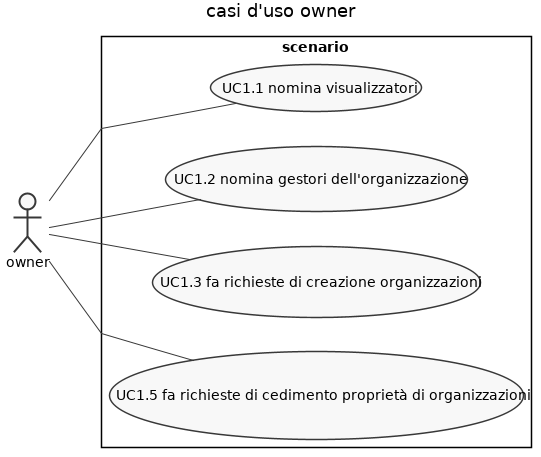
\includegraphics[width=8cm]{owner_use_cases.png}
  \centering
  \caption{diagramma dei casi d'uso realizzato con PlantUml}
\end{figure}

N.B.: la figura~\ref{fig:esempio_caso_duso} è un'immagine, non codice PlantUML.\@ Per vedere un'applicazione pratica di quanto detto, si vedano ad es.\ i diagrammi inclusi nel documento \textit{Analisi dei requisiti}.

In seguito a difficoltà nell'utilizzo del package apposito di \LaTeX{}, abbiamo deciso di pre-compilare separatamente i diagrammi utilizzando le funzionalità esposte dalla \glossario{Command Line Interface} di PlantUML\@.

Eseguendo nella radice del repository il comando

\begin{minted}{bash}
  java \
    -jar \
    $PLANTUML_JAR \
    -checkmetadata \
    -charset UTF-8 \
    -x **/commons/style/*.pu \
    -o img \
    **/**.pu
\end{minted}

vengono generate le immagini dei diagrammi che sono incluse nei documenti.
La corretta esecuzione del comando richiede di aver impostato la variabile d'ambiente \verb|PLANTUML\_JAR| al percorso completo del file \verb|plantuml.jar| reperito dal sito del progetto.

% TODO mancano altri strumenti in questa sezione?

\end{document}
